%
% green.tex
%
% (c) 2019 Prof Dr Andreas Müller, Hochschule Rapperswil
%
\documentclass[tikz,12pt]{standalone}
\usepackage{amsmath}
\usepackage{times}
\usepackage{txfonts}
\usepackage{pgfplots}
\usepackage{csvsimple}
\usetikzlibrary{arrows,intersections,math}
\begin{document}
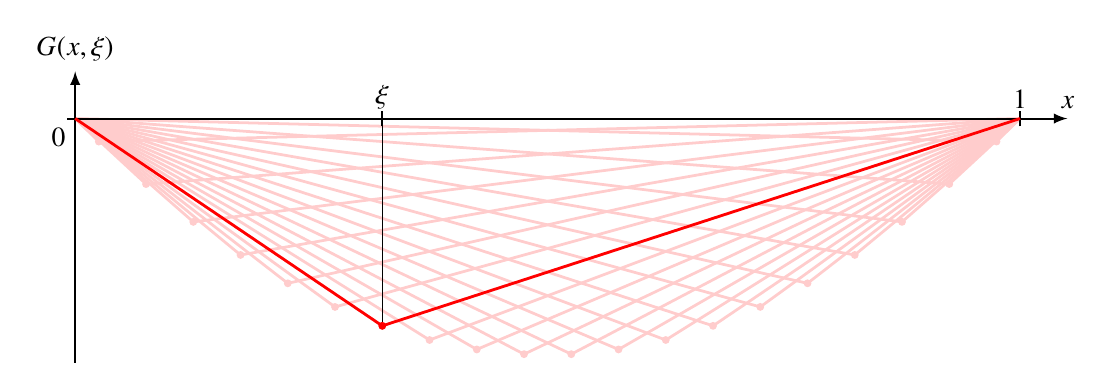
\begin{tikzpicture}[>=latex]

\def\s{12}

\foreach \xi in {0.025,0.075,...,1}{
	\draw[color=red!20,line width=1pt] (0,0)--({\s*\xi},{\s*\xi*(\xi-1)});
	\draw[color=red!20,line width=1pt] ({\s*\xi},{\s*\xi*(\xi-1)})--(\s,0);
	\fill[color=red!20] ({\s*\xi},{\s*\xi*(\xi-1)}) circle[radius=0.05];
}

\draw[->,line width=0.7pt] (-0.1,0)--({\s+0.6},0) coordinate[label=$x$];
\draw[->,line width=0.7pt] (0,{-0.25*\s-0.1})--(0,0.6)
	coordinate[label={$G(x,\xi)$}];

\draw[line width=0.7pt] ({\s},-0.1)--({\s},0.1);
\node at ({\s},0) [above] {$1$};
\node at (0,0) [below left] {$0$};

\def\xiv{0.325}

\draw[line width=0.5pt] ({\s*\xiv},0)--({\s*\xiv},{\s*\xiv*(\xiv-1)});
\draw[line width=0.7pt] ({\s*\xiv},-0.1)--({\s*\xiv},0.1);
\node at ({\s*\xiv},0) [above] {$\xi$};

\draw[color=red,line width=1pt] (0,0)--({\s*\xiv},{\s*\xiv*(\xiv-1)});
\draw[color=red,line width=1pt] ({\s*\xiv},{\s*\xiv*(\xiv-1)})--(\s,0);
\fill[color=red] ({\s*\xiv},{\s*\xiv*(\xiv-1)}) circle[radius=0.05];

\end{tikzpicture}
\end{document}

